\section{Saules paneļi}
% KĀ STRĀDĀ SAULES PANEĻI?
% fotons uzspīd elektronam un viņu ierosina un tad tas aiziet pāri vadītspējas zonai un aizpeld uz elektrodu un caurums aizpeld uz otru elektrodu un rodas potenciālu starpība no kurienes strāva.
% Ielikt dokus par LG un JA tipu + no kādiem kristāliem tie
% Ielikt shēmu
% analīze par saules paneļu plantācijām pasaulē
% optimālie apstākļi?



\begin{figure}[h]
    \centering
    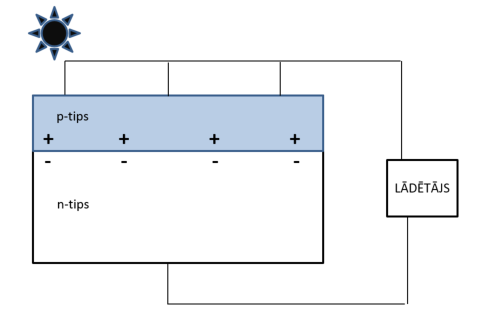
\includegraphics[width=0.7\linewidth]{figures/misc/solar_cell.pdf}
    \caption{Saules paneļa shēma. Tas sastāv no fotoelementiem, kuru augšējais slānis veidots no p-tipa pusvadītāja, bet apakšējais --- no n-tipa pusvadītāja.}
    \label{fig:PV}
\end{figure}
